\chapter{椭圆型方程的离散与线性系统}
\label{ch:discretization}

本章建立后续全书共同使用的离散对象：怎样从连续椭圆型方程得到有限个未知量、局部 stencil 和全局线性系统。后面的 Jacobi、Gauss--Seidel、多重网格以及并行实现都只是在操作这个离散系统，因此第一章最重要的不是记住若干公式，而是能够解释每一个矩阵系数从哪一个局部关系产生。

本章先用 Poisson 方程建立节点型有限差分的最小模型，再保持同一个 Poisson 问题不变，引入 cell-centered 有限体积。这样读者可以先单独理解“方法怎样不同”。随后才把连续模型推广为一般变系数椭圆算子，并要求 FD 与 FV 分别完成一次推广。最后再讨论同一组边界条件怎样进入这两种已经明确的离散表示。两条路线最终都会得到 $A\bm u=\bm b$，但未知量位置和局部方程的生成机制并不相同。\textbf{本章始终只讨论单一分辨率网格}；局部细化以及粗、细离散层之间的耦合留到\chapref{ch:amr-discretization}。

\begin{keybox}
\textbf{本章的核心学习链：}
\[
\boxed{\text{Poisson}\rightarrow
\begin{cases}
\text{节点型 FD：导数近似}\\
\text{cell-centered FV：控制体收支}
\end{cases}
\rightarrow\text{局部离散关系}}
\]
\[
\boxed{\text{一般椭圆算子}\rightarrow
\begin{cases}
\text{FD：半点通量再做散度差分}\\
\text{FV：材料系数进入数值面通量}
\end{cases}
\rightarrow\text{加权局部耦合}}
\]
\[
\boxed{\text{边界数据}\rightarrow\text{按未知量布局闭合}\rightarrow\text{矩阵行/右端/零空间的变化}}
\]
第一次阅读需要始终回答四个问题：当前连续方程是什么？未知量放在哪里？一条局部离散方程是怎样生成的？边界信息最终改变了哪一个代数对象？Kronecker 记号、DtN、张量各向异性以及详细存储预算属于压缩表示或扩展内容，可以跳过而不破坏核心路径。
\end{keybox}

\section{一维 Poisson 方程的离散与线性系统}

\subsection{连续模型与网格}

先考虑最简单的一维模型：在区间 $0<x<L$ 上求函数 $u(x)$，使
\begin{equation}
-\frac{\mathrm d^2u}{\mathrm dx^2}=f(x),
\label{eq:discretization-poisson-one-dimensional}
\end{equation}
并给定两端的函数值
\begin{equation}
u(0)=g_0,\qquad u(L)=g_L.
\label{eq:discretization-dirichlet-one-dimensional}
\end{equation}
式 \eqref{eq:discretization-poisson-one-dimensional} 是一维 Poisson 方程，式 \eqref{eq:discretization-dirichlet-one-dimensional} 是 Dirichlet 边界条件。这里的未知量不是有限个数字，而是整个函数 $u(x)$。计算机最终必须把“求一个函数”转化为“求有限个数”。

为此，把区间划分为等距网格。令
\begin{equation}
x_i=ih,\qquad i=0,1,\ldots,N+1,
\end{equation}
其中
\begin{equation}
h=\frac{L}{N+1}.
\end{equation}
边界点是 $x_0=0$ 与 $x_{N+1}=L$，内部有 $N$ 个网格点。我们用
\begin{equation}
u_i\approx u(x_i)
\end{equation}
表示连续函数在第 $i$ 个网格点上的近似值。

此时问题已经发生第一次变化：原来未知的是整个函数 $u(x)$，现在准备求的是
\begin{equation}
\bm u=(u_1,u_2,\ldots,u_N)^T.
\end{equation}
下一步只需要回答一个问题：连续方程里的二阶导数 $u''(x_i)$，怎样用附近几个 $u_j$ 表示？

\subsection{二阶中心差分}

在 $x_i$ 两侧各取一个网格点。对足够光滑的 $u(x)$，Taylor 展开给出
\begin{align}
u(x_i+h)
&=u(x_i)+h u'(x_i)+\frac{h^2}{2}u''(x_i)
 +\frac{h^3}{6}u^{(3)}(x_i)+\Oh(h^4),\\
u(x_i-h)
&=u(x_i)-h u'(x_i)+\frac{h^2}{2}u''(x_i)
 -\frac{h^3}{6}u^{(3)}(x_i)+\Oh(h^4).
\end{align}
两式相加，一阶导数项和三阶导数项相消：
\begin{equation}
u(x_i+h)-2u(x_i)+u(x_i-h)
=h^2u''(x_i)+\Oh(h^4).
\end{equation}
除以 $h^2$，得到中心差分公式
\begin{equation}
u''(x_i)
=\frac{u(x_i-h)-2u(x_i)+u(x_i+h)}{h^2}+\Oh(h^2).
\label{eq:discretization-second-difference}
\end{equation}
忽略截断误差项，并用网格未知量 $u_{i-1},u_i,u_{i+1}$ 替代连续函数值，就有
\begin{equation}
-u''(x_i)
\approx
\frac{-u_{i-1}+2u_i-u_{i+1}}{h^2}.
\label{eq:discretization-one-dimensional-stencil-equation}
\end{equation}
代回 Poisson 方程：
\begin{equation}
\frac{-u_{i-1}+2u_i-u_{i+1}}{h^2}=f_i,
\qquad f_i=f(x_i).
\label{eq:discretization-one-dimensional-discrete}
\end{equation}

这一步就是\textbf{离散化（discretization）}：把连续微分算子转化为有限个网格值之间的代数关系。式 \eqref{eq:discretization-one-dimensional-discrete} 只依赖当前点和左右相邻点，其局部系数可以记成
\begin{equation}
\frac{1}{h^2}[-1,\;2,\;-1].
\end{equation}
后文把这种固定的局部依赖模式称为\textbf{模板（stencil）}。

\begin{checkpointbox}
\textbf{即时检查}

如果把网格间距从 $h$ 缩小到 $h/2$，中心差分的截断误差主项大约缩小多少倍？式 \eqref{eq:discretization-second-difference} 中的 $\Oh(h^2)$ 已经给出了答案所需的信息。
\end{checkpointbox}

\subsection{一维离散系统与矩阵表示}

取 $N=5$。未知量为
\begin{equation}
\bm u=
\begin{bmatrix}
u_1&u_2&u_3&u_4&u_5
\end{bmatrix}^T.
\end{equation}
对每个内部点应用式 \eqref{eq:discretization-one-dimensional-discrete}：
\begin{align}
\frac{-u_0+2u_1-u_2}{h^2}&=f_1,\\
\frac{-u_1+2u_2-u_3}{h^2}&=f_2,\\
\frac{-u_2+2u_3-u_4}{h^2}&=f_3,\\
\frac{-u_3+2u_4-u_5}{h^2}&=f_4,\\
\frac{-u_4+2u_5-u_6}{h^2}&=f_5.
\end{align}
边界值 $u_0=g_0$ 和 $u_6=g_L$ 已知，因此不属于未知向量。把已知边界项移到右端：
\begin{equation}
\frac1{h^2}
\begin{bmatrix}
2&-1&0&0&0\\
-1&2&-1&0&0\\
0&-1&2&-1&0\\
0&0&-1&2&-1\\
0&0&0&-1&2
\end{bmatrix}
\begin{bmatrix}
u_1\\u_2\\u_3\\u_4\\u_5
\end{bmatrix}
=
\begin{bmatrix}
f_1+g_0/h^2\\
f_2\\
f_3\\
f_4\\
f_5+g_L/h^2
\end{bmatrix}.
\label{eq:discretization-matrix-five}
\end{equation}

现在可以给式 \eqref{eq:discretization-matrix-five} 起统一的名字：
\begin{equation}
A\bm u=\bm b.
\label{eq:discretization-Aub}
\end{equation}
$A$ 是离散算子对应的矩阵，$\bm u$ 是待求的网格未知量，$\bm b$ 包含源项以及由边界条件带来的已知贡献。

\begin{keybox}
不要把 $A\bm u=\bm b$ 当成凭空出现的抽象线性代数记号。对于 Poisson 问题，矩阵的每一行就是某一个网格点上的局部离散方程；矩阵中非零元素的位置，就是 stencil 的邻接关系。
\end{keybox}

\section{二维与三维 Poisson 离散}

一维问题已经给出了完整的离散链条：在每个网格位置写一个局部差分方程，再把所有局部方程按未知量编号组装成全局线性系统。进入二维和三维以后，\textbf{这个原则不变，但“局部邻接怎样变成全局矩阵”第一次变得不再显然}。因此本节不从最一般的公式开始，而是先完整组装一个很小的二维系统，再由这个小系统抽象出二维块结构，最后把同一思路提升到三维切片。

\subsection{二维五点格式}

先考虑正方形区域上的二维 Poisson 方程
\begin{equation}
-\nabla^2u
=-\frac{\partial^2u}{\partial x^2}
 -\frac{\partial^2u}{\partial y^2}
=f(x,y),
\end{equation}
并暂时取两个方向相同的网格间距 $h$。在内部网格点 $(i,j)$，分别沿 $x$、$y$ 方向使用一维中心差分：
\begin{align}
-\frac{\partial^2u}{\partial x^2}
&\approx \frac{2u_{i,j}-u_{i-1,j}-u_{i+1,j}}{h^2},\\
-\frac{\partial^2u}{\partial y^2}
&\approx \frac{2u_{i,j}-u_{i,j-1}-u_{i,j+1}}{h^2}.
\end{align}
两式相加得到
\begin{equation}
\boxed{
\frac{
4u_{i,j}-u_{i-1,j}-u_{i+1,j}-u_{i,j-1}-u_{i,j+1}
}{h^2}
=f_{i,j}.
}
\label{eq:discretization-two-dimensional-five-point}
\end{equation}
这就是二维五点格式。它仍然是一条\textbf{局部方程}：中心未知量只与四个轴向邻居耦合。

\begin{figure}[htbp]
\centering
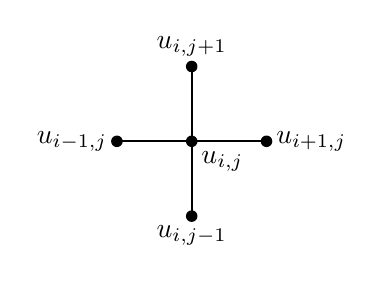
\begin{tikzpicture}[scale=0.95]
  \foreach \x/\y in {0/1,1/0,1/1,1/2,2/1}{\fill (\x,\y) circle (2.2pt);}
  \draw[thick] (0,1)--(2,1);
  \draw[thick] (1,0)--(1,2);
  \node[below] at (1,0) {$u_{i,j-1}$};
  \node[above] at (1,2) {$u_{i,j+1}$};
  \node[left] at (0,1) {$u_{i-1,j}$};
  \node[right] at (2,1) {$u_{i+1,j}$};
  \node[below right] at (1,1) {$u_{i,j}$};
\end{tikzpicture}
\caption{二维五点 stencil。二维化首先改变的是局部邻接：一维的左右两个邻居变成两个坐标方向上的四个邻居。}
\label{fig:discretization-five-point-stencil}
\end{figure}

\subsection{二维局部方程与全局矩阵}

真正需要建立的新心智模型，是二维几何怎样进入一维线性代数向量。先取一个只有 $2\times2$ 个内部未知量的小网格，四周均为齐次 Dirichlet 边界。按
\begin{equation}
\bm u=
\begin{bmatrix}
 u_{1,1}&u_{2,1}&u_{1,2}&u_{2,2}
\end{bmatrix}^{T}
\end{equation}
编号。对四个内部点分别应用式~\eqref{eq:discretization-two-dimensional-five-point}，边界值因为为零直接消失：
\begin{align}
4u_{1,1}-u_{2,1}-u_{1,2}&=h^2f_{1,1},\\
-u_{1,1}+4u_{2,1}-u_{2,2}&=h^2f_{2,1},\\
-u_{1,1}+4u_{1,2}-u_{2,2}&=h^2f_{1,2},\\
-u_{2,1}-u_{1,2}+4u_{2,2}&=h^2f_{2,2}.
\end{align}
于是
\begin{equation}
\boxed{
\frac1{h^2}
\begin{bmatrix}
4&-1&-1&0\\
-1&4&0&-1\\
-1&0&4&-1\\
0&-1&-1&4
\end{bmatrix}
\begin{bmatrix}
u_{1,1}\\u_{2,1}\\u_{1,2}\\u_{2,2}
\end{bmatrix}
=
\begin{bmatrix}
f_{1,1}\\f_{2,1}\\f_{1,2}\\f_{2,2}
\end{bmatrix}.
}
\label{eq:discretization-two-dimensional-small-matrix}
\end{equation}

这个 $4\times4$ 例子暴露了二维化真正新增的结构。矩阵仍然是一行对应一个网格点，但非零元的位置不再只沿主对角线附近连续排列；它们取决于\textbf{二维网格中的几何邻接}以及我们选择的编号方式。

对一般 $n_x\times n_y$ 个内部节点，采用 $x$ 方向先变化的字典序编号
\begin{equation}
p(i,j)=i+n_x(j-1),
\qquad
1\le i\le n_x,
\quad
1\le j\le n_y.
\label{eq:discretization-two-dimensional-indexing}
\end{equation}
于是左右邻居在向量中相差 $1$，上下邻居相差 $n_x$。若网格仍为 $h_x=h_y=h$，把同一条 $x$ 向网格线上的未知量看成一个块，则矩阵具有块三对角结构
\begin{equation}
A_{2D}
=\frac1{h^2}
\begin{bmatrix}
B&-I&&\\
-I&B&\ddots&\\
&\ddots&\ddots&-I\\
&&-I&B
\end{bmatrix},
\qquad
B=\operatorname{tridiag}(-1,4,-1).
\label{eq:discretization-two-dimensional-block-matrix}
\end{equation}
这里的 $B$ 描述同一条水平网格线内部的左右耦合，而块间的 $-I$ 描述相邻两条水平网格线之间的上下耦合。

\begin{keybox}
二维矩阵的块结构不是额外规定出来的。它只是“二维局部邻接 + 一维编号”共同产生的结果。先看懂式~\eqref{eq:discretization-two-dimensional-small-matrix}，再看式~\eqref{eq:discretization-two-dimensional-block-matrix}，就不需要把块三对角结构当成需要背诵的新公式。
\end{keybox}

在这个结构已经清楚以后，矩形网格 $h_x\neq h_y$ 只是把两个方向的权重分开：
\begin{equation}
\boxed{
\frac{2u_{i,j}-u_{i-1,j}-u_{i+1,j}}{h_x^2}
+
\frac{2u_{i,j}-u_{i,j-1}-u_{i,j+1}}{h_y^2}
=f_{i,j}.
}
\label{eq:discretization-two-dimensional-rectangular-grid}
\end{equation}
因此“两个方向具有不同尺度”是对已经理解的二维结构增加不同权重，而不是理解二维离散的起点。

\paragraph{Kronecker 记号。}
若读者熟悉 Kronecker 积，可以把式~\eqref{eq:discretization-two-dimensional-block-matrix}压缩写成
\begin{equation}
A_{2D}=I_y\otimes T_x+T_y\otimes I_x,
\label{eq:discretization-two-dimensional-kronecker}
\end{equation}
其中 $T_x,T_y$ 是对应方向的一维离散算子，$\otimes$ 表示把一维算子组合成块矩阵的 Kronecker 积。这个写法的作用是\textbf{压缩已经理解的结构}，不是建立二维离散所必需的新概念；第一次阅读可以跳过这一式而不影响后文主线。

\subsection{三维七点格式与切片耦合}

三维最自然的入口不是直接写三重索引，而是把计算域看成一叠二维切片。对固定的 $k$，同一个 $z$ 切片内部仍然有二维的四个轴向邻居；此外，每个点还与上一层 $k-1$ 和下一层 $k+1$ 的对应位置耦合。因此在均匀网格上
\begin{equation}
\boxed{
\frac{
6u_{i,j,k}
-u_{i-1,j,k}-u_{i+1,j,k}
-u_{i,j-1,k}-u_{i,j+1,k}
-u_{i,j,k-1}-u_{i,j,k+1}
}{h^2}
=f_{i,j,k}.
}
\label{eq:discretization-three-dimensional-seven-point}
\end{equation}
这就是三维七点格式。

如果一个 $z$ 切片上的二维离散矩阵记为 $A_{xy}$，那么三维系统可以理解为“二维切片之间再形成块三对角耦合”：
\begin{equation}
A_{3D}
=\begin{bmatrix}
A_{xy}+2h^{-2}I&-h^{-2}I&&\\
-h^{-2}I&A_{xy}+2h^{-2}I&\ddots&\\
&\ddots&\ddots&-h^{-2}I\\
&&-h^{-2}I&A_{xy}+2h^{-2}I
\end{bmatrix}.
\label{eq:discretization-three-dimensional-slice-matrix}
\end{equation}
这个式子比直接记一个三重 Kronecker 和更重要：它说明三维并不是“二维公式多两个邻居”而已，而是\textbf{整个二维子系统之间又发生了层间耦合}。

若三个坐标方向的步长分别为 $h_x,h_y,h_z$，则三个方向分别使用对应的逆平方权重：
\begin{align}
(Au)_{i,j,k}
={}&\frac{2u_{i,j,k}-u_{i-1,j,k}-u_{i+1,j,k}}{h_x^2}\\
&+\frac{2u_{i,j,k}-u_{i,j-1,k}-u_{i,j+1,k}}{h_y^2}\\
&+\frac{2u_{i,j,k}-u_{i,j,k-1}-u_{i,j,k+1}}{h_z^2}.
\label{eq:discretization-three-dimensional-rectangular-grid}
\end{align}

把三维网格存进一维数组时当然还需要一个编号，例如
\begin{equation}
p(i,j,k)=i+n_x\bigl[(j-1)+n_y(k-1)\bigr],
\label{eq:discretization-three-dimensional-indexing}
\end{equation}
但这是\textbf{表示层}的问题，而不是七点离散本身的一部分。后面的并行与存储章节会讨论这种编号如何影响连续访问、子域划分和通信；本章此处只需要知道：同一个三维几何邻接在一维向量中会对应不同的索引跨度。

若需要进一步压缩矩阵结构，也可以写成
\begin{equation}
A_{3D}
=I_z\otimes I_y\otimes T_x
+I_z\otimes T_y\otimes I_x
+T_z\otimes I_y\otimes I_x,
\label{eq:discretization-three-dimensional-kronecker}
\end{equation}
但它和二维情形一样只是结构记号；本章的核心是理解“局部七点关系怎样组成切片耦合的全局系统”。

\begin{checkpointbox}
\textbf{即时检查：二维与三维矩阵结构}

回到式~\eqref{eq:discretization-two-dimensional-small-matrix}，逐个指出每个 $-1$ 对应哪一对二维相邻节点。再想象把这个 $2\times2$ 网格复制成两个 $z$ 切片：哪些新增矩阵非零元用于连接两个切片？如果能回答这个问题，就已经掌握了三维切片耦合的核心，而无需先记忆任何 Kronecker 公式。
\end{checkpointbox}




\section{Poisson 的有限体积离散与数值面通量}
\label{sec:discretization-finite-volume}

前两节始终从 Poisson 方程出发，用\textbf{节点型有限差分（finite difference, FD）}近似点上的微分算子。现在保持连续问题不变，只更换离散表示：仍然求解 Poisson 方程，但改用\textbf{单元中心有限体积（cell-centered finite volume, FV）}。本节只讨论规则均匀笛卡尔网格；更一般的网格几何留到后续章节。

这里必须先区分三个对象：连续方程中的\textbf{精确面通量积分}、离散格式中的\textbf{数值面通量}、以及由同一数值面通量在相邻控制体之间反对称装配所得到的\textbf{离散局部守恒}。后文分别用 $Q_{P,f}$ 与 $\widehat Q_{P,f}$ 表示前两者；二者相等只可能出现在特殊解或极限情形中，一般只有一致性意义下的逼近关系。

\subsection{积分恒等式与精确面通量}

仍考虑
\begin{equation}
-\nabla^2u=f.
\label{eq:discretization-poisson-fv-start}
\end{equation}
定义连续通量场
\begin{equation}
\bm q=-\nabla u.
\label{eq:discretization-poisson-flux}
\end{equation}
若 $u\in C^2(\overline V_P)$，则 $\bm q\in C^1(\overline V_P)$，Poisson 方程可写为 $\nabla\cdot\bm q=f$。对控制体 $V_P$ 使用散度定理，得到\textbf{精确积分恒等式}
\begin{equation}
\sum_{f\subset\partial V_P}Q_{P,f}
=
\int_{V_P} f\,\mathrm dV,
\qquad
Q_{P,f}:=\int_f \bm q\cdot\bm n_{P,f}\,\mathrm dA,
\label{eq:discretization-fv-poisson-balance}
\end{equation}
其中 $\bm n_{P,f}$ 是相对于控制体 $P$ 的外法向。注意这里尚未发生离散化：$Q_{P,f}$ 是连续解 $u$ 所决定的精确面通量积分。

若内部面 $f$ 由相邻控制体 $P$ 与 $N$ 共享，则
\begin{equation}
\bm n_{N,f}=-\bm n_{P,f}.
\end{equation}
因此同一个连续通量场在该共享面上满足
\begin{equation}
\boxed{Q_{N,f}=-Q_{P,f}.}
\label{eq:discretization-exact-flux-antisymmetry}
\end{equation}
这是法向定向直接给出的恒等式，而不是经验性的“流出等于流入”。

为了得到代数方程，还必须近似面通量与体积分。若把 $f_P$ 定义为控制体平均
\begin{equation}
\bar f_P:=\frac1{V_P}\int_{V_P}f\,\mathrm dV,
\end{equation}
则右端可以精确写成 $\bar f_PV_P$。实际程序若改用中心点值 $f(\bm x_P)$，这一步就是一个求积近似；对中心对称的规则 cell 且 $f\in C^2$，中点求积满足
\begin{equation}
\int_{V_P}f\,\mathrm dV
=f(\bm x_P)V_P+\Oh(h^2V_P),
\label{eq:discretization-fv-source-quadrature}
\end{equation}
其中 $h$ 表示局部网格尺度。

\subsection{正交网格上的两点数值通量}

现在才引入数值通量。设规则正交网格上的内部面 $f=P|N$ 的中心为 $\bm x_f$，两个 cell center 沿面法向共线，中心距离为 $d_{PN}$，面面积为 $A_f$。以 $P$ 的外法向为定向，定义两点数值通量
\begin{equation}
\boxed{
\widehat Q_{P,f}
:=T_{PN}(u_P-u_N),
\qquad
T_{PN}:=\frac{A_f}{d_{PN}}.
}
\label{eq:discretization-fv-poisson-two-point-flux}
\end{equation}
这里 $u_P,u_N$ 是 cell-centered 离散未知量。在本章的规则均匀网格上，可以把它们理解为对应中心点函数值的近似；若采用 cell-average 作为未知量，对足够光滑的 $u$，中心值与 cell average 的差异同样是二阶量，不改变这里的二阶主阶分析。

式~\eqref{eq:discretization-fv-poisson-two-point-flux}不是由守恒律本身推出的，而是一个\textbf{通量闭合（flux closure）}。在均匀正交网格上，若 $u\in C^3$，以面中心为展开点可得
\begin{equation}
\frac{u_N-u_P}{d_{PN}}
=
\frac{\partial u}{\partial n}(\bm x_f)+\Oh(h^2),
\end{equation}
因此
\begin{equation}
\widehat Q_{P,f}
=Q_{P,f}+\Oh(A_fh^2)
\end{equation}
在面上法向导数足够光滑且面中点求积成立的意义下是一致的。该结论依赖于这里明确给出的正交、对称几何假设；在一般非正交网格上，简单两点公式未必保持同样的一致性阶数。

更重要的是，共享面只能生成\textbf{一个}数值通量，再以相反符号装配到两侧控制体。按同一个 $T_{PN}$ 定义
\begin{equation}
\widehat Q_{N,f}:=T_{PN}(u_N-u_P),
\end{equation}
于是代数上严格有
\begin{equation}
\boxed{
\widehat Q_{N,f}=-\widehat Q_{P,f}.
}
\label{eq:discretization-numerical-flux-antisymmetry}
\end{equation}
当所有内部面都采用这一共享通量约定时，把任意一组相邻控制体的离散方程相加，内部面数值通量会\textbf{精确抵消}。这才是有限体积格式的离散局部守恒性质。它来自数值通量的反对称装配，而不是来自“公式看起来像通量”的直觉。

\begin{figure}[htbp]
\centering
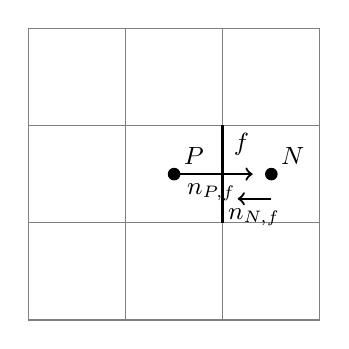
\begin{tikzpicture}[scale=0.95,font=\small]
  \draw[gray] (0,0) grid[step=1.3] (3.9,3.9);
  \fill (1.95,1.95) circle (2.4pt) node[above right] {$P$};
  \fill (3.25,1.95) circle (2.4pt) node[above right] {$N$};
  \draw[very thick] (2.6,1.3)--(2.6,2.6);
  \node[right] at (2.62,2.35) {$f$};
  \draw[->,thick] (1.95,1.95)--(3.0,1.95);
  \node[below] at (2.45,1.95) {$\bm n_{P,f}$};
  \draw[->,thick] (3.25,1.62)--(2.80,1.62);
  \node[below] at (3.02,1.62) {$\bm n_{N,f}$};
\end{tikzpicture}
\caption{共享内部面的定向。连续精确通量满足 $Q_{N,f}=-Q_{P,f}$；离散时若两侧使用同一个共享数值通量，则 $\widehat Q_{N,f}=-\widehat Q_{P,f}$ 也在代数上严格成立。}
\label{fig:discretization-fv-cell-face}
\end{figure}

\subsection{一维 cell-centered Poisson 与一致性}

设一维均匀 cell 宽度为 $h$，第 $i$ 个 cell center 为 $x_i$，左右边界分别为 $x_{i-1/2}$ 与 $x_{i+1/2}$。相对于 cell $i$ 的外法向，数值通量定义为
\begin{align}
\widehat Q_{i,L}&=\frac{u_i-u_{i-1}}{h},\\
\widehat Q_{i,R}&=\frac{u_i-u_{i+1}}{h}.
\end{align}
采用中点求积近似体源，离散平衡写成
\begin{equation}
\widehat Q_{i,L}+\widehat Q_{i,R}=f_i h.
\end{equation}
除以 $h$ 得到
\begin{equation}
\boxed{
\frac{-u_{i-1}+2u_i-u_{i+1}}{h^2}=f_i.
}
\label{eq:discretization-fv-one-dimensional-poisson}
\end{equation}

这一式与节点型中心差分具有相同的代数模板，但其一致性仍需独立验证。把精确解 $u(x_i)$ 代入左端，Taylor 展开给出
\begin{equation}
\frac{-u(x_i-h)+2u(x_i)-u(x_i+h)}{h^2}
=-u''(x_i)-\frac{h^2}{12}u^{(4)}(x_i)+\Oh(h^4).
\end{equation}
因此若 $u\in C^6$，内部离散的局部截断误差为 $\Oh(h^2)$。这说明这里的二阶结论来自 Taylor 展开，而不是来自“FV 与 FD 看起来相同”。

\begin{warningbox}
\textbf{代数模板相同不等于离散对象相同。}

节点型 FD 的未知量位于节点；本节的 cell-centered FV 未知量位于 cell center。即使两者在均匀网格上写出同一个三对角系数模式，它们一般对应不同的物理采样位置。只有在明确给定网格映射、系数位置和右端求积以后，才有资格比较两个离散算子是否代数等价。
\end{warningbox}

\subsection{二维与三维逐面装配}

对二维规则矩形 cell $P$，记四个内部面对应的邻居为 $E,W,N,S$。每个共享面只计算一次数值通量，并按相反符号装配到相邻两个控制体。于是 cell $P$ 的离散方程为
\begin{equation}
\boxed{
\left(T_E+T_W+T_N+T_S\right)u_P
-T_Eu_E-T_Wu_W-T_Nu_N-T_Su_S
=f_PV_P.
}
\label{eq:discretization-fv-poisson-two-dimensional-row}
\end{equation}
在边长为 $h$、单位厚度的均匀正方形网格上，$A_f=h$、$d_{PN}=h$，故 $T_f=1$。再除以 $V_P=h^2$，得到标准五点 Laplacian。这个结论的条件是：规则笛卡尔几何、两点数值通量、中点源项求积以及内部 cell；少掉其中任一条件，都不能直接把“五点格式”当作普遍结论。

三维规则立方体同理，多出上、下两个共享面。若所有六个面都满足同样的正交两点闭合，便得到七点模板。二维到三维真正保持不变的严格结构是：\textbf{每个共享面对应一个反对称的数值通量贡献}；五点或七点只是这一结构在规则笛卡尔网格上的特例。

\subsection{有限差分与有限体积：比较已经证明的内容}

在当前假设下，两种方法可以作如下比较：
\begin{center}
\small
\begin{tabularx}{0.96\textwidth}{>{\bfseries}p{2.7cm}X X}
\toprule
 & 节点型有限差分（FD） & cell-centered 有限体积（FV）\\
\midrule
未知量位置 & 网格节点 & 控制体中心\\
局部方程来源 & 微分算子的差分近似 & 控制体积分恒等式 + 数值面通量闭合\\
首先近似的对象 & 点上的导数 & 面通量积分与体积分\\
二阶结论的依据 & Taylor 截断误差分析 & 通量/求积一致性与等价模板的 Taylor 分析\\
离散局部守恒 & 一般不由“FD”名称自动保证 & 若共享面使用单一反对称数值通量，则严格成立\\
规则 Poisson & 三点/五点/七点 & 在上述假设下得到相同系数模板\\
\bottomrule
\end{tabularx}
\end{center}

下一节把连续模型推广到变系数椭圆算子。届时必须继续区分“连续物理通量”和“人为选择的数值通量”，并检查后者的一致性与共享面反对称性。


\section{从 Poisson 到一般椭圆算子}
\label{sec:discretization-general-elliptic}

考虑标量扩散型算子
\begin{equation}
\mathcal Lu
:=-\nabla\cdot\bigl(\beta(\bm x)\nabla u\bigr)
+\alpha(\bm x)u
=f.
\label{eq:discretization-general-diffusion}
\end{equation}
为了使本节讨论确实处在标准椭圆框架内，先明确基本假设：区域内部取
\begin{equation}
0<\beta_0\le \beta(\bm x)\le \beta_1<\infty,
\qquad
\alpha(\bm x)\ge0,
\label{eq:discretization-ellipticity-assumption}
\end{equation}
并在当前规则网格的一致性分析中假设 $\beta$、$\alpha$ 与精确解具有所需的光滑性。系数跳变时应把问题理解为分片光滑椭圆方程，并额外满足界面条件；该情形不在本节用一个未经证明的“平均公式”代替。

当 $\beta=1$、$\alpha=0$ 时，式~\eqref{eq:discretization-general-diffusion}退化为 Poisson 方程。本节只研究规则均匀笛卡尔网格，目标是严格说明：面/半点系数如何进入离散算子，以及在什么条件下 FD 与 FV 会得到同一代数模板。

\subsection{有限差分：数值半点通量与一致性}

先看一维
\begin{equation}
-\frac{\mathrm d}{\mathrm dx}
\left(\beta(x)\frac{\mathrm du}{\mathrm dx}\right)
+\alpha(x)u
=f.
\label{eq:discretization-general-diffusion-one-dimensional}
\end{equation}
定义连续通量
\begin{equation}
F(x):=-\beta(x)u'(x),
\end{equation}
则方程为 $F'(x)+\alpha(x)u(x)=f(x)$。在均匀节点 $x_i=ih$ 上，定义\textbf{数值半点通量}
\begin{equation}
\widehat F_{i+1/2}
:=-\beta_{i+1/2}\frac{u_{i+1}-u_i}{h},
\label{eq:discretization-fd-variable-face-flux}
\end{equation}
并取离散散度
\begin{equation}
\frac{\widehat F_{i+1/2}-\widehat F_{i-1/2}}{h}
+\alpha_i u_i
=f_i.
\label{eq:discretization-fd-variable-divergence}
\end{equation}

这里的关键不是把 $\widehat F$ 称为“通量”，而是验证它是否一致。若 $u\in C^5$，在半点 $x_{i+1/2}$ 展开可得
\begin{equation}
\frac{u(x_{i+1})-u(x_i)}{h}
=u'(x_{i+1/2})
+\frac{h^2}{24}u^{(3)}(x_{i+1/2})
+\Oh(h^4).
\label{eq:discretization-centered-first-derivative-midpoint}
\end{equation}
若同时
\begin{equation}
\beta_{i+1/2}
=\beta(x_{i+1/2})+\Oh(h^2),
\label{eq:discretization-face-beta-consistency}
\end{equation}
则
\begin{equation}
\widehat F_{i+1/2}
=F(x_{i+1/2})+\Oh(h^2).
\end{equation}
再对相邻半点的通量作中心差分，Taylor 展开得到
\begin{equation}
\frac{\widehat F_{i+1/2}-\widehat F_{i-1/2}}{h}
=F'(x_i)+\Oh(h^2),
\end{equation}
所以在上述光滑性与面系数一致性条件下，内部离散是二阶一致的。

代入数值通量后得到
\begin{equation}
\boxed{
-\frac{\beta_{i-1/2}}{h^2}u_{i-1}
+\left(
\frac{\beta_{i-1/2}+\beta_{i+1/2}}{h^2}
+\alpha_i
\right)u_i
-\frac{\beta_{i+1/2}}{h^2}u_{i+1}
=f_i.
}
\label{eq:discretization-fd-variable-row}
\end{equation}

这也解释了为什么不能把原算子替换为 $-\beta_i u''$：一般有
\begin{equation}
-(\beta u')'=-\beta u''-\beta'u',
\end{equation}
后者比 $-\beta u''$ 多出一阶耦合项。只有当 $\beta$ 为常数时，两者才相同。

二维均匀笛卡尔网格上，对两个坐标方向分别使用同样的半点构造可得
\begin{align}
&-\frac{
\beta_{i+1/2,j}(u_{i+1,j}-u_{i,j})
-\beta_{i-1/2,j}(u_{i,j}-u_{i-1,j})
}{h_x^2} \\
&-\frac{
\beta_{i,j+1/2}(u_{i,j+1}-u_{i,j})
-\beta_{i,j-1/2}(u_{i,j}-u_{i,j-1})
}{h_y^2}
+\alpha_{i,j}u_{i,j}
=f_{i,j}.
\label{eq:discretization-fd-variable-two-dimensional}
\end{align}
其二阶一致性同样依赖于各方向面系数满足相应的二阶近似条件，而不是只由“五点邻接”这一拓扑事实保证。

\subsection{有限体积：精确积分式、数值通量与求积}

对式~\eqref{eq:discretization-general-diffusion} 在控制体 $V_P$ 上积分，得到精确关系
\begin{equation}
\sum_{f\subset\partial V_P}Q_{P,f}
+
\int_{V_P}\alpha u\,\mathrm dV
=
\int_{V_P}f\,\mathrm dV,
\label{eq:discretization-fv-balance-exact-general}
\end{equation}
其中
\begin{equation}
Q_{P,f}
:=-\int_f\beta\nabla u\cdot\bm n_{P,f}\,\mathrm dA
\label{eq:discretization-bc-flux-definition}
\end{equation}
是连续精确面通量积分。

在本章的均匀正交网格上，定义共享内部面的数值通量
\begin{equation}
\boxed{
\widehat Q_{P,f}
:=T_{PN}(u_P-u_N),
\qquad
T_{PN}:=\frac{\beta_fA_f}{d_{PN}}.
}
\label{eq:discretization-fv-two-point-flux}
\end{equation}
这里要求相邻两个控制体对同一面使用同一个 $\beta_f$ 和同一个 $T_{PN}$，从而严格保持
\begin{equation}
\widehat Q_{N,f}=-\widehat Q_{P,f}.
\label{eq:discretization-fv-general-antisymmetry}
\end{equation}
若 $\beta$ 在面附近光滑，$\beta_f=\beta(\bm x_f)+\Oh(h^2)$，且网格正交对称，则该两点通量对精确面通量是二阶一致的。若 $\beta$ 在面上跳变，则必须由界面连续条件和一侧/两侧系数共同构造 $T_{PN}$；本节不把算术平均或调和平均当作无需条件的定理。

对体积分采用中点求积，
\begin{align}
\int_{V_P}\alpha u\,\mathrm dV
&=\alpha_Pu_PV_P+\Oh(h^2V_P),\\
\int_{V_P}f\,\mathrm dV
&=f_PV_P+\Oh(h^2V_P),
\end{align}
于是得到离散控制体方程
\begin{equation}
\sum_{f\subset\partial V_P}\widehat Q_{P,f}
+\alpha_PV_Pu_P
=f_PV_P.
\label{eq:discretization-fv-balance-general}
\end{equation}
这里的等号定义的是\textbf{离散格式}，不是对连续积分式逐项精确替换。

对二维矩形内部 cell $P$，装配四个共享面的数值通量得到
\begin{equation}
\boxed{
\begin{aligned}
&\left(T_E+T_W+T_N+T_S+\alpha_PV_P\right)u_P\\
&\qquad -T_Eu_E-T_Wu_W-T_Nu_N-T_Su_S
=f_PV_P.
\end{aligned}
}
\label{eq:discretization-two-dimensional-flux-row}
\end{equation}
三维规则笛卡尔网格同理增加上、下两个面。只要同一内部面在两侧使用同一个数值通量，局部守恒是代数恒等式；至于该数值通量是否高阶逼近连续通量，则是另一项必须独立验证的一致性问题。

\subsection{FD 与 FV 的代数重合：条件与边界}

一维均匀网格上，若 FD 与 FV 使用同一组 $\beta_{i\pm1/2}$，FV 采用中点体积分求积，并把每个 cell 的积分方程除以体积 $h$，则两者都得到
\begin{equation}
-\frac{\beta_{i-1/2}}{h^2}u_{i-1}
+\left(
\frac{\beta_{i-1/2}+\beta_{i+1/2}}{h^2}
+\alpha_i
\right)u_i
-\frac{\beta_{i+1/2}}{h^2}u_{i+1}
=f_i.
\end{equation}

这是一个有明确前提的代数结论，而不是“FD 与 FV 本质相同”。至少有三点不能由该式推出：第一，节点型 FD 与 cell-centered FV 的未知量通常位于不同物理位置；第二，在非正交网格或不同求积/重构下，两者未必生成同一矩阵；第三，FV 的共享面反对称装配提供离散局部守恒，而一般 FD 格式是否具有相同性质必须从其具体数值通量形式单独检查。

\subsection{零阶项与零空间}

式~\eqref{eq:discretization-general-diffusion} 中的 $\alpha u$ 不产生新的空间邻居。在节点型 FD 中，它给矩阵对角元增加 $\alpha_i$；在 cell-centered FV 的积分方程中，它贡献 $\alpha_PV_P$。因此在当前点值/中点求积离散下，零阶项不改变内部邻接拓扑。

对连通网格上的纯 Neumann Poisson 离散，扩散部分具有常数零空间。若离散的 $\alpha_i\ge0$，且至少一个自由度上 $\alpha_i>0$（FV 中相应为 $\alpha_iV_i>0$），则常数向量不再属于零空间；在对称扩散离散下，这一事实还可通过离散能量式严格证明。后面的线性代数部分会再次使用这一结构。

\subsection{各向异性算子：由交叉导数说明邻接扩大}

若扩散系数推广为对称正定张量 $\bm B$，考虑常系数二维算子
\begin{equation}
-\nabla\cdot(\bm B\nabla u),
\qquad
\bm B=
\begin{bmatrix}
\beta_{xx}&\beta_{xy}\\
\beta_{xy}&\beta_{yy}
\end{bmatrix}.
\end{equation}
直接展开得
\begin{equation}
-\beta_{xx}u_{xx}
-2\beta_{xy}u_{xy}
-\beta_{yy}u_{yy}.
\label{eq:discretization-anisotropic-expanded}
\end{equation}
若 $\beta_{xy}\ne0$，标准二阶中心差分对 $u_{xy}$ 的近似为
\begin{equation}
u_{xy}(x_i,y_j)
\approx
\frac{
u_{i+1,j+1}-u_{i+1,j-1}-u_{i-1,j+1}+u_{i-1,j-1}}{4h_xh_y},
\end{equation}
它显式引入四个对角邻居。因此在坐标轴不与张量主方向对齐时，经典轴向五点 stencil 一般不足以表示这一标准二阶离散。这一结论来自交叉导数的具体离散式，而不是对“各向异性更复杂”的直观判断。

\begin{keybox}
本节需要保留的严格区分是：\textbf{连续通量}由 PDE 定义，\textbf{数值通量}由离散方法选择；共享面数值通量的反对称性保证\textbf{离散守恒}，而数值通量逼近连续通量的阶数决定\textbf{一致性}。这三个概念不能互相替代。
\end{keybox}

\section{边界条件的离散闭合}
\label{sec:discretization-boundary-conditions}

现在节点型 FD 和 cell-centered FV 都已经建立。连续边界条件本身并不会因为离散方法改变，但它进入代数系统的方式取决于\textbf{未知量布局}：FD 可能在边界节点上直接保存 $u$，FV 则通常通过控制体的边界面提供通量闭合。因此本节不再切换离散表示，只研究“同一个边界信息在已经确定的表示中怎样闭合方程”。本节始终沿着同一条链路：
\begin{equation}
\boxed{
\begin{gathered}
\text{连续边界条件}\longrightarrow\text{离散边界关系}\\
\downarrow\\[-0.4em]
\text{消去边界/辅助量}\longrightarrow\text{修改矩阵行与右端}
\end{gathered}
}
\label{eq:discretization-bc-chain}
\end{equation}
先在一维节点型有限差分上把这条链走通，再进入二维、三维。这样多维边界不会变成一组需要背诵的特殊规则。


\subsection{未知量布局与边界表示}

在写任何边界公式之前，先把两种表示放在一起：
\begin{center}
\small
\begin{tabularx}{0.95\textwidth}{>{\bfseries}p{2.8cm}X X}
\toprule
 & 节点型 FD & cell-centered FV\\
\midrule
边界附近未知量 & 边界点可能就是一个 $u_0$ & 最近未知量在边界内侧的 cell center $P$\\
Dirichlet & 可直接给边界节点值，或消去该自由度 & 用已知边界面值闭合 $Q_f$\\
Neumann & 用单边/辅助点关系近似法向导数 & 直接给定边界面通量或由导数换算通量\\
二维角部 & 不同边界段可能落到同一个角节点 & 一个角部 cell 拥有多个物理边界面\\
三维棱/角 & 一个节点可能位于多个边界面的闭包上 & 一个 cell 可同时拥有两个或三个边界面\\
\bottomrule
\end{tabularx}
\end{center}

因此边界条件离散的第一步永远不是“套 Dirichlet/Neumann 公式”，而是先确认当前代数未知量与物理边界之间的几何关系。

\subsection{一维边界闭合}

回到一维 Poisson 方程。第一个内部点满足
\begin{equation}
\frac{-u_0+2u_1-u_2}{h^2}=f_1.
\label{eq:discretization-bc-first-row-open}
\end{equation}
如果 $u_0$ 既不是已知量，也没有包含在未知向量中，这一行就没有闭合。边界条件的数值作用正是补上关于 $u_0$ 的关系。

有两种常见代数布局：
\begin{enumerate}
\item \textbf{消去边界自由度。}未知向量只保存内部点，用边界条件把 $u_0$ 写成内部未知量和已知数据，再代回式~\eqref{eq:discretization-bc-first-row-open}；
\item \textbf{保留边界自由度。}把 $u_0$ 也放进未知向量，并把离散边界条件本身作为矩阵的一行。
\end{enumerate}
本章首先采用第一种方式，因为它与前面的一维未知向量定义一致。第二种方式在需要保留边界节点时也很常见，两者的区别是\textbf{未知量布局}，不是连续边界条件本身发生了变化。

\subsection{Dirichlet 边界条件}

左端 Dirichlet 条件直接给定
\begin{equation}
u_0=g_D.
\end{equation}
代入式~\eqref{eq:discretization-bc-first-row-open}：
\begin{equation}
\boxed{
\frac{2u_1-u_2}{h^2}
=f_1+\frac{g_D}{h^2}.
}
\label{eq:discretization-dirichlet-row}
\end{equation}
所以 Dirichlet 条件没有增加未知量，而是把原来 stencil 中的边界值移入右端。若边界自由度被保留，则还可以直接使用
\begin{equation}
u_0=g_D
\end{equation}
作为边界行；如果后续算法依赖矩阵对称性，强制单位行时还应同时处理对应矩阵列，或者直接消去该自由度。

\subsection{Neumann 边界条件}

Neumann 条件给定外法向导数
\begin{equation}
\frac{\partial u}{\partial n}=g_N.
\label{eq:discretization-neumann-bc}
\end{equation}
左端点的外法向指向 $-x$，因此
\begin{equation}
-u'(0)=g_N.
\end{equation}
用最简单的一阶差分
\begin{equation}
u'(0)\approx\frac{u_1-u_0}{h}
\end{equation}
得到
\begin{equation}
u_0=u_1+h g_N.
\label{eq:discretization-neumann-eliminate-uzero}
\end{equation}
代回第一行：
\begin{equation}
\boxed{
\frac{u_1-u_2}{h^2}
=f_1+\frac{g_N}{h}.
}
\label{eq:discretization-neumann-first-row}
\end{equation}
与 Dirichlet 相比，第一行的对角系数已经发生变化。边界条件因此不仅改变右端，也可能改变矩阵本身。

例如左端取 Neumann、右端取 Dirichlet $u_{N+1}=g_R$。未知向量仍由内部值 $u_1,\ldots,u_N$ 组成，此时矩阵变为
\begin{equation}
\frac1{h^2}
\begin{bmatrix}
1&-1&&&\\
-1&2&-1&&\\
&\ddots&\ddots&\ddots&\\
&&-1&2&-1\\
&&&-1&2
\end{bmatrix}
\begin{bmatrix}
u_1\\u_2\\\vdots\\u_{N-1}\\u_N
\end{bmatrix}
=
\begin{bmatrix}
f_1+g_N/h\\f_2\\\vdots\\f_{N-1}\\f_N+g_R/h^2
\end{bmatrix}.
\label{eq:discretization-mixed-neumann-dirichlet-matrix}
\end{equation}

\paragraph{纯 Neumann 情形。}
若两端都给 Neumann 条件，矩阵两端的对角元都变成 $1/h^2$。齐次情形下常数向量满足
\begin{equation}
A\bm 1=0,
\end{equation}
因此解只确定到一个加法常数。连续方程相应要求兼容条件
\begin{equation}
\boxed{
\int_\Omega f\,\mathrm d\Omega
+\int_{\partial\Omega}g_N\,\mathrm dS=0.
}
\label{eq:discretization-neumann-compatibility}
\end{equation}
这里的零空间不是求解器制造出来的，而是边值问题本身的一部分；后面的迭代方法必须尊重这一结构。

\subsection{Robin 边界条件}

Robin 条件给定函数值与外法向导数的局部线性组合：
\begin{equation}
a u+b\frac{\partial u}{\partial n}=g.
\label{eq:discretization-robin-general}
\end{equation}
仍看左端。用
\begin{equation}
\frac{\partial u}{\partial n}
\approx
\frac{u_0-u_1}{h}
\end{equation}
得到
\begin{equation}
(ah+b)u_0-bu_1=gh,
\end{equation}
于是
\begin{equation}
\boxed{
u_0=\frac{b}{ah+b}u_1+\frac{gh}{ah+b}.
}
\label{eq:discretization-robin-boundary-value}
\end{equation}
代回式~\eqref{eq:discretization-bc-first-row-open}：
\begin{equation}
\boxed{
\frac{2ah+b}{h^2(ah+b)}u_1
-\frac1{h^2}u_2
=f_1+\frac{g}{h(ah+b)}.
}
\label{eq:discretization-robin-matrix-row}
\end{equation}
当 $b=0$ 时得到 Dirichlet 型闭合；当 $a=0$ 时得到 Neumann 型闭合。这个极限检查比死记 Robin 行更重要，因为它能直接发现符号或法向约定写错的问题。

到这里，一维中最常见的三种局部边界条件已经完成了同一件事：\textbf{把缺失的边界信息转化成一条闭合的矩阵行。}

\begin{warningbox}
\textbf{边界闭合的精度必须单独检查。}

上面的 Neumann 和 Robin 推导刻意使用一阶单边导数，只为了让“边界关系怎样进入矩阵行”完全透明。它并不自动与内部二阶中心差分组成整体二阶格式。若目标是保持二阶精度，应改用二阶单边差分、与目标阶数一致的边界闭合，或在有限体积中采用与目标阶数一致的边界通量重构。\textbf{内部 stencil 的阶数不能替代边界离散的阶数检查。}
\end{warningbox}

\subsection{二维边界段与角点}

二维新增的困难不是“多写一个 $y$ 方向导数”，而是\textbf{不同边界段会在角点相遇}。先继续使用前面的节点型有限差分布局。设矩形区域的西、东、南、北四条边分别记为
\begin{equation}
\Gamma_W,\quad\Gamma_E,\quad\Gamma_S,\quad\Gamma_N.
\end{equation}
每一条开放边界段内部都可以使用前面的一维法向离散；真正的新问题出现在边界段的交界。

\paragraph{两个 Dirichlet 边界相交。}
若西边给
\begin{equation}
u(0,y)=g_W(y)
\end{equation}
而南边给
\begin{equation}
u(x,0)=g_S(x),
\end{equation}
那么左下角只有一个几何点 $(0,0)$。如果要求连续解具有连续的边界迹（trace，即把域内解限制到边界后得到的值），自然需要
\begin{equation}
g_W(0)=g_S(0).
\label{eq:discretization-dirichlet-corner-compatibility}
\end{equation}
在节点型离散中，角点也只对应一个节点，因此程序最终必须给它一个唯一值。需要注意的是：如果只要求积分意义上的弱解，单个几何角点的数据不一定像整段边界数据那样决定域内解；本章不展开这一函数空间问题。对离散程序而言，只要网格显式保存该角点，就仍然必须给它一个唯一、明确的离散值。

\paragraph{Dirichlet 与 Neumann 相交。}
若西边是 Dirichlet、南边是 Neumann，一个常见的节点型约定是：角点值由 Dirichlet 条件确定，而 Neumann 条件施加在南边界除该角点以外的边界节点上。比如南边界外法向为 $-y$，用一阶法向差分时，对 $i\ge1$ 的南边界节点可写
\begin{equation}
u_{i,0}=u_{i,1}+h\,g_S(x_i),
\end{equation}
而左下角直接取
\begin{equation}
u_{0,0}=g_W(0).
\end{equation}
这样不会给同一个角点未知量同时写两条独立边界行。这个规则是\textbf{离散约定}，不是所有方法都必须采用的唯一处理方式；有限元、有限体积或不同的边界辅助点构造可以采用不同布局。

\paragraph{边界类型改变与解的光滑性。}
即使每条边界数据本身合法，Dirichlet--Neumann 或 Dirichlet--Robin 的切换点也可能降低局部正则性（也就是解的光滑程度）；几何再入角会进一步加强这种效应。第一章不展开椭圆正则性理论，只保留一个数值后果：\textbf{内部 stencil 是二阶的，并不自动保证含边界交界的整个问题仍表现出理想的二阶全局收敛。}验证时必须把交界附近误差也包含在网格收敛测试中。

三维的结构是同一问题的进一步提升：边界条件定义在二维面上，两个面在棱上相遇，三个面在角点相遇。节点型离散若显式保存这些棱/角节点，就必须给出一致的交界约定；这不是把二维角点规则逐字复制三遍，而是同一个未知量可能同时落在更多边界片段的闭包上。

\begin{figure}[htbp]
\centering
\begin{tikzpicture}[scale=0.88,font=\small]
  % nodal panel
  \begin{scope}[xshift=0cm]
    \draw[very thick] (0,0)--(0,2.2);
    \draw[very thick] (0,0)--(2.2,0);
    \foreach \x in {0,0.8,1.6}{
      \foreach \y in {0,0.8,1.6}{\fill (\x,\y) circle (2pt);}
    }
    \draw[gray] (0,0.8)--(1.6,0.8) (0,1.6)--(1.6,1.6)
                (0.8,0)--(0.8,1.6) (1.6,0)--(1.6,1.6);
    \filldraw[fill=white,draw=black,thick] (0,0) circle (3.4pt);
    \node[above left] at (0,0) {角节点};
    \node[left] at (0,1.25) {$\Gamma_D$};
    \node[below] at (1.2,0) {$\Gamma_N$};
    \node at (0.8,-0.65) {节点型：保存角节点};
  \end{scope}
  % cell-centered panel
  \begin{scope}[xshift=5.4cm]
    \draw[very thick] (0,0)--(0,2.2);
    \draw[very thick] (0,0)--(2.2,0);
    \draw[gray] (0,1)--(2,1) (1,0)--(1,2) (0,2)--(2,2) (2,0)--(2,2);
    \foreach \x/\y in {0.5/0.5,1.5/0.5,0.5/1.5,1.5/1.5}{\fill (\x,\y) circle (2.2pt);}
    \node[above right] at (0.5,0.5) {$P$};
    \node[above right] at (1.5,0.5) {$E$};
    \node[above right] at (0.5,1.5) {$N$};
    \node[left] at (0,0.5) {$f_W$};
    \node[below] at (0.5,0) {$f_S$};
    \node at (1.0,-0.65) {cell-centered：边界面闭合};
  \end{scope}
\end{tikzpicture}
\caption{同一个二维物理角在两种离散布局中的不同代数对象。左：节点型有限差分显式保存角节点；右：cell-centered 有限体积没有角点未知量，角部控制体 $P$ 通过西、南两个边界面接收边界贡献。}
\label{fig:discretization-corner-layouts}
\end{figure}

\begin{center}
\footnotesize
\begin{tabularx}{0.92\textwidth}{>{\bfseries}p{3.0cm}X X}
\toprule
二维交界 & 节点型离散需要决定什么 & 连续/数值上应检查什么\\
\midrule
Dirichlet--Dirichlet & 同一个角节点只能取一个值 & 经典连续 trace 是否一致；离散数据冲突时必须给出唯一约定\\
Dirichlet--Neumann/\newline Robin & 常见做法是由 Dirichlet 固定角节点，另一条件作用于开放边界段 & 交界附近正则性与整体收敛阶\\
Neumann--Neumann & 两条边给出不同法向分量，角节点仍需具体 closure & 全局兼容条件、角部离散精度与零空间\\
Robin--Robin /\newline Neumann--Robin & 一个节点同时邻接两条局部边界关系 & 采用何种角点方程必须由离散布局明确，而不能机械叠加两条矩阵行\\
\bottomrule
\end{tabularx}
\end{center}

\subsection{cell-centered 有限体积中的边界面}
\label{sec:discretization-cell-centered-boundary}

对边界 cell，连续精确通量仍定义为
\begin{equation}
Q_{P,f}=-\int_f\beta\frac{\partial u}{\partial n}\,\mathrm dA,
\end{equation}
其中法向始终取\textbf{相对于控制体 $P$ 的外法向}。边界条件的作用，是给这个缺少相邻 cell 的面提供一个数值通量 $\widehat Q_{P,f}$。为了避免符号混乱，下面所有 Neumann 数据 $g_N$ 均定义为
\begin{equation}
\frac{\partial u}{\partial n}=g_N
\end{equation}
中的\textbf{外法向导数}；因此对应的连续外向扩散通量是 $-\beta g_N$，不是 $+\beta g_N$。

\paragraph{Dirichlet 面：一侧两点闭合。}
若边界面给定 $u_f=g_D$，cell center 到边界面的法向距离为 $\delta_f$，最简单的两点闭合是
\begin{equation}
\widehat Q_{P,f}
=T_f(u_P-g_D),
\qquad
T_f=\frac{\beta_fA_f}{\delta_f}.
\label{eq:discretization-bc-dirichlet-numerical-flux}
\end{equation}
这只是一个数值通量定义。若 $u_P$ 解释为中心点值，则 $(g_D-u_P)/\delta_f$ 对边界法向导数通常只有一阶一致性；因此不能仅凭内部二阶 stencil 宣称整个边值问题二阶收敛。高阶边界闭合必须另行构造和分析。

\paragraph{Neumann 面：通量由边界数据直接给出。}
若 $\partial_nu=g_N$，并以面中点值代表边界数据，则
\begin{equation}
\boxed{
\widehat Q_{P,f}=-\beta_fA_fg_N.
}
\label{eq:discretization-bc-neumann-numerical-flux}
\end{equation}
若 $g_N$ 或 $\beta$ 沿面变化，更严格的表达应是对 $-\beta g_N$ 的面求积；上式本身包含中点求积近似。

考虑二维左下角控制体 $P$：西面为 Dirichlet $u=g_D$，南面为 Neumann $\partial_nu=g_N$，东、北分别邻接内部 cell $E,N$。将四个面的数值通量代入
\begin{equation}
\sum_f\widehat Q_{P,f}+\alpha_PV_Pu_P=f_PV_P
\end{equation}
得到
\begin{equation}
\boxed{
\begin{aligned}
&\left(T_{PE}+T_{PN}+T_W+\alpha_PV_P\right)u_P
-T_{PE}u_E-T_{PN}u_N\\
&\qquad =f_PV_P+T_Wg_D+\beta_SA_Sg_N.
\end{aligned}
}
\label{eq:discretization-mixed-corner-row}
\end{equation}
右端出现 $+\beta_SA_Sg_N$ 的原因不是人为规定符号，而是 Neumann 面的外向数值通量为 $-\beta_SA_Sg_N$，移到方程右端后符号改变。

\paragraph{一般仿射边界闭合。}
若边界面数值关系可写成
\begin{equation}
u_f=c_fu_P+s_f,
\label{eq:discretization-bc-affine-closure}
\end{equation}
并仍采用
\begin{equation}
\widehat Q_{P,f}
=T_f(u_P-u_f),
\qquad
T_f=\frac{\beta_fA_f}{\delta_f},
\label{eq:discretization-bc-transmissibility}
\end{equation}
则代数上严格有
\begin{equation}
\widehat Q_{P,f}
=T_f(1-c_f)u_P-T_fs_f.
\end{equation}
把已知项移到右端后，该边界面对矩阵与右端的贡献为
\begin{equation}
\boxed{
\Delta A_{PP}=T_f(1-c_f),
\qquad
\Delta b_P=T_fs_f.
}
\label{eq:discretization-bc-general-matrix-contribution}
\end{equation}
这只是给定离散边界闭合后的代数恒等式；其准确度由 $u_f=c_fu_P+s_f$ 本身的截断误差决定。

对 Robin 条件
\begin{equation}
a_fu_f+b_f\frac{\partial u}{\partial n}=g_f,
\end{equation}
若使用一阶法向近似
\begin{equation}
\frac{\partial u}{\partial n}
\approx\frac{u_f-u_P}{\delta_f},
\end{equation}
且 $a_f\delta_f+b_f\ne0$，则
\begin{equation}
u_f
=\frac{b_f}{a_f\delta_f+b_f}u_P
+\frac{g_f\delta_f}{a_f\delta_f+b_f},
\end{equation}
从而
\begin{equation}
\boxed{
\Delta A_{PP}
=\frac{\beta_fA_fa_f}{a_f\delta_f+b_f},
\qquad
\Delta b_P
=\frac{\beta_fA_fg_f}{a_f\delta_f+b_f}.
}
\label{eq:discretization-robin-matrix-contribution}
\end{equation}
令 $b_f=0$ 可检查 Dirichlet 极限，令 $a_f=0$ 可检查 Neumann 极限；但这种极限检查只能验证代数与符号的一致性，不能替代边界截断误差分析。

对一个控制体 $P$，记 $\mathcal N(P)$ 为内部面邻居集合，$\Gamma(P)$ 为物理边界面集合，则
\begin{equation}
\boxed{
\begin{aligned}
&\left(
\alpha_PV_P
+\sum_{N\in\mathcal N(P)}T_{PN}
+\sum_{f\in\Gamma(P)}\Delta A_f
\right)u_P\\
&\qquad
-\sum_{N\in\mathcal N(P)}T_{PN}u_N
=
f_PV_P
+\sum_{f\in\Gamma(P)}\Delta b_f.
\end{aligned}
}
\label{eq:discretization-general-boundary-row}
\end{equation}
该式是给定内部数值通量与边界数值通量之后的装配公式。它本身不提供收敛阶；收敛阶必须结合内部一致性、边界一致性、稳定性以及问题正则性共同判断。

\begin{keybox}
\textbf{FV 边界面的符号规则只有一条：先固定外法向，再定义外向数值通量。}

Dirichlet、Neumann、Robin 的矩阵符号都应从 $\widehat Q_{P,f}$ 推导，而不是分别背诵。特别地，若 Neumann 数据定义为 $\partial_nu=g_N$，则外向扩散通量为 $-\beta g_N$；将该已知通量移到右端后才出现 $+\beta A g_N$。
\end{keybox}

\subsection{周期边界条件}

周期条件不是给定一个已知边界值或通量，而是把一侧的未知量与另一侧对应位置识别为同一个周期邻居。对一维周期网格，令
\begin{equation}
u_0=u_N,
\qquad
u_{N+1}=u_1.
\end{equation}
则矩阵成为循环三对角结构：
\begin{equation}
\frac1{h^2}
\begin{bmatrix}
2&-1&0&\cdots&-1\\
-1&2&-1&&0\\
0&\ddots&\ddots&\ddots&\vdots\\
\vdots&&-1&2&-1\\
-1&0&\cdots&-1&2
\end{bmatrix}.
\label{eq:discretization-periodic-matrix}
\end{equation}
所以周期条件的代数特征是\textbf{新增跨边界的未知量耦合}，而不是把已知数据移到右端。没有零阶项时，周期 Poisson 与纯 Neumann 一样具有常数零空间。

二维若只在 $x$ 方向周期，每一条固定 $j$ 的网格线都在左右边界之间建立邻接；若 $x,y$ 两个方向都周期，则角部邻接同时跨越两个方向。三维中，一个周期面要按两个切向坐标与对侧面逐点配对；当两个或三个方向同时周期时，来自不同方向的映射还必须在棱和角处组成一致的等价关系。这里的核心仍然是“修改邻接关系”；具体跨边界数据访问与通信实现留到\chapref{ch:parallel-model}之后的并行章节。

\subsection{Dirichlet-to-Neumann 算子}

前面的 Dirichlet、Neumann 和 Robin 都是局部边界关系。DtN 不同：它来自被截去的外部区域，一般把\textbf{整段或整个边界上的函数值}映射为相应的法向响应，因此通常是非局部算子。本小节属于扩展内容；第一次阅读只需掌握“外域可以被消去，并在边界上留下一个矩阵算子”这一点。

为了避免导数与物理扩散通量之间的符号混乱，这里把离散 DtN 直接定义成\textbf{边界值到外向扩散通量}的映射：
\begin{equation}
\bm q_\Gamma
=K_\Gamma\bm u_\Gamma+\bm q_\Gamma^{(0)}.
\label{eq:discretization-discrete-dtn-flux}
\end{equation}
若 $C_\Gamma\bm u$ 提取全局未知量在边界上的 trace，而 $B_\Gamma$ 把边界通量装配进相邻方程，则
\begin{equation}
A_{int}\bm u+B_\Gamma\bm q_\Gamma=\bm b_{int}
\end{equation}
变成
\begin{equation}
\boxed{
\left(A_{int}+B_\Gamma K_\Gamma C_\Gamma\right)\bm u
=
\bm b_{int}-B_\Gamma\bm q_\Gamma^{(0)}.
}
\label{eq:discretization-dtn-matrix-form}
\end{equation}
如果 $K_\Gamma$ 只是逐点乘法，这个边界修改看起来像局部 Robin；一般二维、三维外域中，$K_\Gamma$ 会耦合多个边界自由度，因此边界块可以明显宽于原来的局部 stencil。

\paragraph{一个可精确求出的模型外域。}
为把 DtN 从抽象矩阵变成可手算对象，考虑内部区域 $0<x<L$，
\begin{equation}
-u''=f,
\qquad
u(0)=g_0,
\end{equation}
而外部半直线 $x>L$ 满足
\begin{equation}
-v''+\kappa^2v=0,
\qquad
v(x)\to0\quad(x\to\infty),
\qquad
v(L)=u(L),
\end{equation}
其中 $\kappa>0$。这个 modified Helmholtz 外域被选来作为教学模型，是因为它具有显式衰减解；\textbf{它不是一般静电 Poisson 外域的普遍 DtN 公式。}

外域解为
\begin{equation}
v(x)=u(L)e^{-\kappa(x-L)},
\end{equation}
于是内部区域右端外法向为 $+x$ 时
\begin{equation}
\boxed{
\frac{\partial u}{\partial n}(L)=-\kappa u(L).
}
\label{eq:discretization-dtn-one-dimensional-exact}
\end{equation}
若扩散系数为 $\beta$，对应外向扩散通量为 $q=\beta\kappa u(L)$，因此在前面“值到通量”的定义下，这个一维 DtN 只是标量 $K_\Gamma=[\beta\kappa]$。

下面为了得到一个完整矩阵，\textbf{切换回节点型有限差分}，并让 $u_N$ 本身位于截断边界 $x=L$。取 $x_i=ih$、$L=Nh$，未知向量为
\begin{equation}
\bm u=(u_1,\ldots,u_N)^T.
\end{equation}
内部节点 $i=1,\ldots,N-1$ 使用
\begin{equation}
-u_{i-1}+2u_i-u_{i+1}=h^2f_i,
\end{equation}
而边界导数用一阶后向差分：
\begin{equation}
\frac{u_N-u_{N-1}}{h}=-\kappa u_N.
\end{equation}
因此最后一行是
\begin{equation}
-u_{N-1}+(1+\kappa h)u_N=0,
\end{equation}
完整系统为
\begin{equation}
\boxed{
\begin{bmatrix}
2&-1&0&\cdots&0\\
-1&2&-1&\ddots&\vdots\\
0&\ddots&\ddots&\ddots&0\\
\vdots&\ddots&-1&2&-1\\
0&\cdots&0&-1&1+\kappa h
\end{bmatrix}
\begin{bmatrix}
u_1\\u_2\\\vdots\\u_{N-1}\\u_N
\end{bmatrix}
=
\begin{bmatrix}
h^2f_1+g_0\\h^2f_2\\\vdots\\h^2f_{N-1}\\0
\end{bmatrix}.
}
\label{eq:discretization-dtn-one-dimensional-matrix}
\end{equation}
这个例子说明：外部半无限区域已经从未知量中消失，但它留下了一个边界矩阵行。这里 DtN 恰好具有 Robin 形式，不是因为 DtN 与 Robin 一般等价，而是因为这个一维外域的消去结果恰好是局部标量关系。

\paragraph{外域消元与 Schur 补。}
一般情况下，可以把完整离散系统按内部未知量和外部未知量分块：
\begin{equation}
\begin{bmatrix}
A_{II}&A_{IE}\\
A_{EI}&A_{EE}
\end{bmatrix}
\begin{bmatrix}
\bm u_I\\\bm u_E
\end{bmatrix}
=
\begin{bmatrix}
\bm b_I\\\bm b_E
\end{bmatrix}.
\end{equation}
消去 $\bm u_E$ 得到
\begin{equation}
\boxed{
\left(A_{II}-A_{IE}A_{EE}^{-1}A_{EI}\right)\bm u_I
=
\bm b_I-A_{IE}A_{EE}^{-1}\bm b_E.
}
\label{eq:discretization-dtn-schur}
\end{equation}
这就是 DtN 非局部性的离散来源：即使 $A_{EE}$ 本身稀疏，$A_{EE}^{-1}$ 一般仍是全局的。

\begin{checkpointbox}
\textbf{即时检查：DtN 的一维模型}

只把式~\eqref{eq:discretization-dtn-one-dimensional-exact} 看成边界算子族 $u'(L)+\kappa u(L)=0$，考察 $\kappa\to0^+$ 时最后一行趋向什么局部条件。注意：这只是边界算子族的代数极限；把原来的衰减外域方程直接设成 $\kappa=0$ 会使“任意非零边界值并在无穷远衰减”这一外域问题退化。
\end{checkpointbox}

\subsection{边界条件对线性系统的影响}

现在可以把本节压缩成一张代数地图：
\begin{center}
\small
\begin{tabularx}{0.96\textwidth}{>{\bfseries}p{2.5cm}X X}
\toprule
边界类型 & 闭合机制 & 对 $A\bm u=\bm b$ 的主要影响\\
\midrule
Dirichlet & 给定边界值 & 消去后修改相邻行与右端；保留边界节点时可写边界约束行。\\
Neumann & 给定外法向导数/通量 & 通常改变边界附近行并引入已知通量；纯 Neumann 保留常数零空间。\\
Robin & 值与法向导数的局部线性组合 & 同时改变边界附近矩阵系数和右端。\\
Periodic & 把对侧位置识别为邻居 & 新增跨边界 off-diagonal coupling；多方向周期还要求角/棱映射一致。\\
DtN & 用外域消元得到边界算子 & 一般产生非局部边界耦合，可理解为外域 Schur 补。\\
\bottomrule
\end{tabularx}
\end{center}

\begin{keybox}
\textbf{边界条件最终必须回答两个问题：}

第一，连续边界信息怎样闭合靠近边界的离散方程？

第二，闭合以后究竟修改了哪些未知量、矩阵系数、右端项、零空间或邻接关系？

二维和三维真正新增的难点，是多个边界片段会在角、棱处相遇，而且不同离散布局对这些几何对象的表示不同。
\end{keybox}



\section{离散线性系统的结构性质}

\subsection{稀疏性}

到这里，我们已经用 FD 与 FV 两种表示离散了 Poisson，并把两条路线都推广到变系数椭圆算子，再加入多种边界闭合。现在从线性代数视角检查这些离散系统共同保留下来的结构。对最基本的一维 Poisson，若有 $N$ 个内部点，矩阵尺寸是 $N\times N$，但三点 stencil 使每一行通常只有三个非零元素；二维五点与三维七点格式也只耦合有限数量的邻居。一般变系数算子虽然会改变局部系数，只要离散仍保持局部耦合，稀疏结构就会保留下来。

这种“矩阵尺寸很大，但绝大部分元素都是零”的结构称为\textbf{稀疏（sparse）}。例如三维 $100^3$ 网格有
\begin{equation}
N=10^6
\end{equation}
个未知量。若把 $A$ 当成普通稠密矩阵，它有 $10^{12}$ 个位置；而七点 stencil 真正产生的非零耦合数量只有 $\Oh(N)$ 量级。

因此稀疏性不是某种存储技巧人为制造出来的，而是 PDE 局部性的全局线性代数表现：\textbf{一个局部微分算子只把每个未知量与有限数量的邻居耦合，所以组装后的大矩阵仍然只含有限数量的局部连接。}

这个结论也解释了为什么上一节的边界条件会影响稀疏结构。普通 Dirichlet、Neumann、Robin 和周期条件只增加或修改有限范围内的耦合；而精确 DtN 一般是非局部的，离散后可能在边界自由度之间引入远距离耦合，使边界块比普通 stencil 更稠密。

\subsection{对称性}

回到一维 Dirichlet Poisson 的矩阵。式 \eqref{eq:discretization-matrix-five} 中
\begin{equation}
A^T=A.
\end{equation}
也就是说，$A_{ij}=A_{ji}$。这称为\textbf{对称矩阵（symmetric matrix）}。

这一性质可以直接由装配式验证：若内部共享面 $f=P|N$ 使用同一个 $T_{PN}=T_{NP}$，则 $P$ 行中 $N$ 列与 $N$ 行中 $P$ 列都等于 $-T_{PN}$。因此在未按不同 cell 体积重新缩放各行、且边界消元保持对称处理的前提下，内部面装配保留矩阵对称性。若对不同体积的控制体逐行除以 $V_P$，Euclidean 内积下的矩阵一般不再由这一论证自动保证对称；此时应转而考察加权内积或重新缩放后的算子。

边界实现却可能改变这一性质。例如保留 Dirichlet 边界自由度时，如果只把边界行强行替换成单位行，却不相应消去或修改其他行中的该边界列，那么得到的代数矩阵一般不再对称。需要 SPD 结构时，通常使用自由度消去或对行、列进行一致的对称处理。由此可见，\textbf{“连续算子自伴”并不保证任何随手写出的边界矩阵都自动对称。}

\subsection{正定性与半正定性}

对任意非零向量 $\bm x\in\R^N$，若
\begin{equation}
\bm x^TA\bm x>0,
\qquad \bm x\neq0,
\end{equation}
则称 $A$ 为\textbf{正定矩阵（positive definite）}。

对于一维 Dirichlet Poisson 的三对角矩阵，去掉共同的 $1/h^2$ 后有
\begin{equation}
\bm x^TA\bm x
=\frac1{h^2}\left[
 x_1^2
 +\sum_{i=1}^{N-1}(x_{i+1}-x_i)^2
 +x_N^2
\right].
\label{eq:discretization-discrete-energy}
\end{equation}
右边是若干平方项之和。只要 $\bm x\neq0$，该表达式就严格大于零。因此这个矩阵既对称又正定，简称\textbf{SPD（symmetric positive definite）}。

对于带 Dirichlet 边界的标准 Poisson 离散，上式给出严格正定性。纯 Neumann 情形则不同：常数向量属于零空间，因此二次型可以等于零但不会为负，此时离散算子是\textbf{对称半正定（symmetric positive semidefinite）}。这与前面纯 Neumann 问题“解只确定到一个常数”的结论是同一件事在线性代数中的表达。

本章只需要掌握对称、正定与半正定的基本含义。它们为什么会影响迭代方法和多重网格收敛，将在后续章节真正需要时再讨论。

\begin{checkpointbox}
\textbf{即时检查}

根据式 \eqref{eq:discretization-discrete-energy}，为什么 Dirichlet Poisson 不可能存在一个非零向量 $\bm x$ 使 $A\bm x=0$？提示：若 $A\bm x=0$，则 $\bm x^TA\bm x$ 等于多少？
\end{checkpointbox}


\section{显式矩阵与 Matrix-Free 算子}

得到 $A\bm u=\bm b$ 后，程序必须回答一个非常具体的问题：\textbf{应用 $A$ 时，算子信息究竟存在哪里？}显式矩阵和 matrix-free 的差异，本质上是两种不同的算子表示方式，而不是两个不同的数学问题。

\subsection{显式稀疏矩阵的存储对象}

显式方法把非零矩阵系数真正保存下来。以常见的 CSR（Compressed Sparse Row）思想为例，一个稀疏矩阵至少需要三类数组：
\begin{enumerate}
\item \texttt{values}：所有非零矩阵元素的数值；
\item \texttt{column\_index}：每个非零元素属于哪一列；
\item \texttt{row\_pointer}：每一行的非零元素在前两个数组中的起止位置。
\end{enumerate}

对三维七点离散，内部行大约有七个非零元素。若有 $N$ 个未知量，则
\begin{equation}
\mathrm{nnz}\approx7N,
\end{equation}
其中 $\mathrm{nnz}$ 表示 nonzeros，即非零元素总数。边界会让实际数量略小，但不改变量级。

显式矩阵的优势是结构完全自描述：一个通用稀疏线性代数程序只看这些数组，就能知道每个未知量与哪些列耦合、耦合系数是多少。代价是：\textbf{不仅要存系数，还要存“这些系数属于哪里”的索引信息。}

对于规则 stencil，也可以采用固定对角线、固定邻居等更紧凑的显式格式，从而省掉部分索引。但只要把每个局部系数预先物化并长期保存，它仍属于显式算子表示。

\subsection{Matrix-Free 的存储对象}

Matrix-free 不保存通用的 $(A_{ij})$ 非零列表，而是保存“生成这些局部系数所需要的信息”，并在应用算子时现场计算。

三维常系数 Poisson 是最极端的例子。若网格间距固定，算子只需要知道
\begin{equation}
h_x,\quad h_y,\quad h_z
\end{equation}
以及边界条件等少量元数据，就可以从固定七点公式计算 $Au$。此时没有必要保存 $7N$ 个系数，更没有必要保存 $7N$ 个列索引。

但 matrix-free 并不等于“算子不占内存”。对更一般的式 \eqref{eq:discretization-general-diffusion}，可能仍需保存：
\begin{itemize}
\item cell-centered 的 $\alpha_i$；
\item 各方向 face-centered 的 $\beta$；
\item 网格尺寸或几何信息；
\item 边界类型、边界值或边界 mask；
\item 不规则几何下的体积分数、面积分数或其他局部几何系数。
\end{itemize}
区别在于，这些数据描述的是\textbf{物理/几何系数}，而不是每一个矩阵非零元及其列号。

\begin{keybox}
\textbf{两种表示方式到底存什么：}

显式稀疏矩阵存“已经组装好的代数耦合”：$A_{ij}$ 及其稀疏位置。

Matrix-free 存“生成代数耦合所需的规则和系数”：网格、材料参数、边界与局部几何；$A_{ij}$ 在执行 $Au$ 时临时产生。
\end{keybox}

\subsection{算子存储与工作向量}

比较内存时必须把两类东西分开：
\begin{equation}
\boxed{
\text{总内存}
=\text{算子表示}
+\text{未知量/右端/残差等工作向量}
+\text{求解器额外工作区}.
}
\end{equation}

无论显式还是 matrix-free，至少都要保存未知量 $u$ 和右端 $b$。迭代求解时通常还会有残差 $r=b-Au$、临时向量和其他求解器工作区；残差与迭代修正将在\chapref{ch:iterative-smoothing}正式建立。因此不能把“matrix-free 不存矩阵”误解成“整个求解只需要一个 $u$ 数组”。

为了把问题说清楚，先只比较单层三维七点问题，并假设所有标量均为 FP64，即每个数占 $8$ byte。

若保留四个 cell-centered 向量
\begin{equation}
u,\quad b,\quad r,\quad w,
\end{equation}
其共同内存为
\begin{equation}
M_{vec}=4\times8N=32N\ \text{byte}.
\label{eq:discretization-vector-memory}
\end{equation}
这部分是两种表示都可能需要的共同成本。

\subsection{三维七点算子的存储预算}

现在给出一个具体预算。取
\begin{equation}
N=256^3=16{,}777{,}216
\end{equation}
个未知量。忽略边界辅助层、内存对齐、容器元数据和求解器额外工作区，只估算最核心的数据。

\paragraph{显式 CSR。}
假设内部每行近似 $7$ 个非零元，矩阵数值用 FP64，列索引用 32-bit integer，row pointer 用 64-bit integer。则
\begin{align}
M_{value}
&\approx7N\times8
=56N\ \text{byte}, \\
M_{col}
&\approx7N\times4
=28N\ \text{byte}, \\
M_{row}
&\approx(N+1)\times8
\approx8N\ \text{byte}.
\end{align}
所以仅矩阵本身约为
\begin{equation}
\boxed{
M_{CSR}\approx92N\ \text{byte}
}
\label{eq:discretization-csr-memory}
\end{equation}
代入 $N=256^3$，约为
\begin{equation}
896\ \mathrm{MiB}
+448\ \mathrm{MiB}
+128\ \mathrm{MiB}
=1472\ \mathrm{MiB}
\approx1.44\ \mathrm{GiB}.
\end{equation}
再加式 \eqref{eq:discretization-vector-memory} 中四个工作向量的 $512\ \mathrm{MiB}$，已经接近
\begin{equation}
1.94\ \mathrm{GiB}.
\end{equation}
这还没有计算边界辅助层、内存对齐、容器元数据或求解器额外工作区。

\paragraph{常系数 Matrix-Free。}
对规则三维 Poisson，算子本身只需要少量网格步长和边界元数据。与 $N$ 成正比的主要成本就是工作向量，因此上述四个 FP64 向量约为
\begin{equation}
\boxed{512\ \mathrm{MiB}}.
\end{equation}
与通用 CSR 相比，差异并不是“少了七个浮点数”这么简单，还同时少了列索引和行指针。

\paragraph{变系数 Matrix-Free。}
若保存一个 cell-centered $\alpha$ 和三个方向的 face-centered $\beta$，在大规则三维网格上可粗略估为
\begin{equation}
N+3N=4N
\end{equation}
个 FP64 系数，即约
\begin{equation}
32N\ \text{byte}=512\ \mathrm{MiB}.
\end{equation}
再加四个工作向量，总核心数据约为
\begin{equation}
1.0\ \mathrm{GiB}.
\end{equation}
这已经明显高于常系数 matrix-free，却仍低于上述通用 CSR 示例。若 $\beta$ 是常数，则三个面系数数组又可以退化为少量标量。

\begin{table}[htbp]
\centering
\small
\begin{tabularx}{0.94\textwidth}{>{\raggedright\arraybackslash}p{3.7cm}
                                  >{\raggedright\arraybackslash}X
                                  >{\raggedleft\arraybackslash}p{2.4cm}}
\toprule
表示方式 & 主要存储对象 & $256^3$ 示例\\
\midrule
显式 CSR 算子 & 非零值、列索引、行指针 & 约 $1.44\ \mathrm{GiB}$\\
四个公共工作向量 & $u,b,r,w$ & $0.50\ \mathrm{GiB}$\\
常系数 matrix-free 算子 & 网格步长、边界等少量元数据 & 相对可忽略\\
变系数 matrix-free 算子 & $\alpha$ 与三个方向 face coefficient & 约 $0.50\ \mathrm{GiB}$\\
\bottomrule
\end{tabularx}
\caption{三维七点问题的核心存储预算。该表刻意不计边界辅助层、内存对齐、容器元数据和求解器额外工作区，因此是理解量级的预算而非具体程序的峰值 RSS。}
\label{tab:discretization-storage-budget}
\end{table}

\begin{warningbox}
\textbf{不要把上述预算当成任何库的固定内存公式。}
索引宽度、边界行、稀疏格式、系数是否共享、边界辅助层宽度、工作向量数量和求解器额外工作区都会改变实际 RSS。这里的目标是建立预算方法：先数“每个未知量需要多少 value、多少 index、多少辅助向量”，再乘以 $N$。
\end{warningbox}

\subsection{表示方式的工程取舍}

显式矩阵的主要优势是通用性。矩阵一旦组装完成，许多不依赖几何信息的稀疏线性代数算法可以直接使用它；如果同一个矩阵会被反复求解，组装成本也可以摊薄。

Matrix-free 的主要优势是减少算子存储和内存流量，并避免把一个本来由简单局部公式定义的算子重复编码成“数值 + 索引”。代价是每次应用算子时需要重新计算局部系数或 stencil；而某些只接受显式矩阵的代数算法也无法直接使用。

因此二者不是“先进方法与落后方法”的关系。判断标准是：
\begin{equation}
\boxed{
\begin{gathered}
\text{算子结构是否可由较少的几何/物理信息重建，}\\
\text{以及后续算法是否必须访问显式矩阵条目。}
\end{gathered}
}
\end{equation}

对规则低阶 Poisson/扩散算子，matrix-free 往往非常自然；对一般非结构稀疏系统，显式稀疏矩阵则提供更通用的接口。后面的性能章节还会进一步看到：存储预算不仅决定“能不能装进内存”，也决定一次 $Au$ 需要从内存系统搬运多少字节。


\begin{keybox}
\textbf{关于局部网格细化的前向提示：}本章所有 stencil 都建立在同一离散层上。如果只在局部区域使用更细的网格，新的困难不只是把 $h$ 换成更小的数；粗、细网格会在分辨率交界处相遇，必须重新回答“界面通量如何守恒”“细网格缺失的邻居值从哪里来”“被细网格覆盖的粗网格未知量是否仍是独立自由度”等问题。\chapref{ch:amr-discretization}将从这些问题出发构造自适应网格上的复合离散系统。
\end{keybox}

\section{本章小结}

本章建立了“连续方程--离散算子--线性系统”的完整链条。关键术语如下：

\begin{center}
\begin{tabularx}{0.94\textwidth}{>{\bfseries}p{3.0cm}X}
\toprule
术语 & 本章需要掌握的含义\\
\midrule
网格（grid） & 用有限个空间位置代表连续区域。\\
stencil & 一个网格点的离散方程依赖哪些邻居，以及这些邻居以什么局部系数参与。\\
离散化 & 把连续微分方程转化为有限个代数方程。\\
有限体积（FV） & 从控制体积分恒等式出发，以数值面通量和体积分求积闭合 cell-centered 离散方程。\\
transmissibility & 在给定网格与通量闭合下，把面面积、中心距离和面系数组合成数值面通量权重；其适用性必须由几何与一致性条件保证。\\
稀疏矩阵 & 大部分矩阵元素为零；PDE 局部离散天然产生这种结构。\\
Dirichlet 条件 & 在边界给定函数值。\\
Neumann 条件 & 在边界给定法向导数。\\
Robin 条件 & 在同一边界点给定函数值与法向导数的局部线性组合。\\
DtN 算子（扩展） & 把整个边界上的 Dirichlet 数据映射为相应的 Neumann 数据；一般是非局部边界算子。\\
SPD & 矩阵同时对称且正定。\\
零空间 & 所有满足 $A\bm z=0$ 的向量组成的集合。\\
显式稀疏矩阵 & 保存已经组装好的非零系数及其稀疏位置；CSR 是一种常见表示。\\
Matrix-free（工程扩展） & 不显式保存完整矩阵，而是保存生成局部系数所需的网格、材料与边界信息。\\
一般椭圆算子 & $-\nabla\cdot(\beta\nabla u)+\alpha u=f$；在 $\beta\ge\beta_0>0$ 等条件下属于标准扩散型椭圆算子，离散时必须分别验证面系数/数值通量的一致性。\\
\bottomrule
\end{tabularx}
\end{center}

到这里，读者应能够完成五件可以直接检验的工作。第一，从一维 Poisson 方程推导节点型有限差分并组装小型矩阵；第二，从二维小网格解释五点邻接怎样形成块三对角结构，并把三维看成二维切片之间的进一步耦合；第三，对同一个 Poisson 方程区分精确面通量与数值面通量，从控制体积分恒等式推导 cell-centered FV，并证明共享面数值通量的反对称装配如何给出离散局部守恒；第四，对一般算子 $-\nabla\cdot(\beta\nabla u)+\alpha u=f$，在明确的光滑性、椭圆性与规则网格假设下分别建立 FD 与 FV，并用截断误差说明二阶一致性成立的条件；第五，针对 Dirichlet、Neumann、Robin、周期以及扩展的 DtN，先固定法向与未知量布局，再从离散关系推导矩阵行、右端与零空间，而不是依据直观判断符号和阶数。

在此基础上，变系数算子不再只是“把常数换成数组”：空间变化的 $\beta$ 进入面/半点连接权重，零阶项 $\alpha u$ 则主要增加本地对角贡献。显式矩阵与 matrix-free 一节进一步说明这些数学对象在程序中分别保存什么。具体界面离散、复合网格、迭代求解器、多重网格粗化和并行框架将在后续章节逐步引入。

\section*{习题}

本章习题按“手算离散 $\rightarrow$ 推导结构 $\rightarrow$ 编程验证 $\rightarrow$ 工程判断”组织。计算题应写出中间步骤，不只给最终结论。

\subsection*{计算题}
\begin{enumerate}[label=\arabic*.]
\item 取 $u(x)=e^x$，在 $x=0.5$ 处分别用 $h=0.2,0.1,0.05$ 的三点中心差分近似 $u''(x)$。计算每个 $h$ 下的绝对误差，并用相邻两组误差估计实验收敛阶。
\item 对边值问题
\[
-u''=1,\qquad 0<x<1,\qquad u(0)=0,\quad u(1)=1,
\]
取 $h=1/4$。以三个内部节点值为未知量，写出完整的 $A\bm u=\bm b$，并用消元法求出离散解。将结果与连续精确解在三个节点处比较。
\item 对
\[
-u''=x,\qquad u(0)=1,\qquad u'(1)=2,
\]
取 $h=1/4$。内部点使用二阶中心差分，右端 Neumann 条件使用一阶后向差分。以 $u_1,u_2,u_3,u_4$ 为未知量，逐行写出 $4\times4$ 矩阵和右端向量。
\item 对右端 Robin 条件
\[
2u(1)+3u'(1)=5,
\]
取 $h=1/4$，用一阶后向差分离散导数。把边界方程写成矩阵最后一行；再分别令 Robin 系数退化到纯 Dirichlet 与纯 Neumann，检查矩阵最后一行怎样变化。
\item 对一维截断外域问题，已知精确 DtN 为 $u'(L)=-\kappa u(L)$。取 $L=1$、$h=1/3$、$\kappa=2$、左端 $u(0)=0$，内部方程为 $-u''=1$。写出完整离散线性系统并求解。
\item 在一维均匀网格的某个内部位置，给定 $h=1/2$、$\beta_{i-1/2}=2$、$\beta_{i+1/2}=5$、$\alpha_i=3$。分别从式~\eqref{eq:discretization-fd-variable-row}和 FV 的逐面收支写出该位置的离散行，并比较左右邻居系数、对角系数和右端缩放。
\item 对 $4\times4$ 个内部节点的二维 Poisson 五点离散，采用 lexicographic ordering。写出矩阵的 block-tridiagonal 结构，明确主块和相邻块；计算矩阵阶数与非零元数量。
\item 对一个二维左下角 cell-centered 控制体，西侧给 Dirichlet $u=2$，南侧给外法向 Neumann $\partial_nu=3$，东、北 transmissibility 均为 1，西侧 transmissibility 为 2，南侧 $\beta A=4$，且 $fV=5$。使用式~\eqref{eq:discretization-mixed-corner-row}写出该矩阵行的数值系数和右端。
\item 考虑一个三维 cell-centered 角部控制体 $P$。其东、北、上三个内部面 transmissibility 均为 1；西面为 Dirichlet $u=2$ 且 $T_W=2$；南面为 Neumann $\partial_nu=3$ 且 $\beta A=4$；下面为 Robin $2u+\partial_nu=5$，取 $\delta=1/2$ 且 $\beta A=2$；另有 $fV=1$、$\alpha=0$。逐面计算三个物理边界的矩阵/右端贡献，并写出 $P$ 行。解释为什么这里不是给几何角点写三条独立边界方程。
\item 对 $n_x=n_y=n_z=2$ 的三维内部网格，利用式~\eqref{eq:discretization-three-dimensional-kronecker}写出 $8\times8$ 七点 Poisson 矩阵的块结构，并指出 $x,y,z$ 三个方向邻居在一维编号中的跨度。
\end{enumerate}

\subsection*{推导与证明题}
\begin{enumerate}[label=\arabic*.]
\item 用 Taylor 展开推导三点中心差分二阶导数公式，并严格得到截断误差的 $\Oh(h^2)$ 主项。
\item 从精确积分恒等式~\eqref{eq:discretization-fv-poisson-balance}与数值通量~\eqref{eq:discretization-fv-poisson-two-point-flux}出发，对一维均匀 cell-centered 网格推导式~\eqref{eq:discretization-fv-one-dimensional-poisson}。明确区分 $Q_{P,f}$ 与 $\widehat Q_{P,f}$，并证明式~\eqref{eq:discretization-numerical-flux-antisymmetry}使任意内部共享面在全局求和时精确抵消。最后用 Taylor 展开验证内部离散的二阶局部截断误差。
\item 从式~\eqref{eq:discretization-centered-first-derivative-midpoint}和条件~\eqref{eq:discretization-face-beta-consistency}出发，证明数值半点通量 $\widehat F_{i+1/2}$ 对连续通量 $F(x_{i+1/2})$ 二阶一致，并进一步推导守恒型 FD 行~\eqref{eq:discretization-fd-variable-row}的二阶局部截断误差。再从 FV 离散式~\eqref{eq:discretization-fv-balance-general}说明，在同一均匀网格、同一面系数和同一中点求积下为何会得到相同代数行。
\item 对一维零 Dirichlet Poisson 离散矩阵证明
\[
\bm v^T A\bm v
=\frac{1}{h^2}\sum_i (v_i-v_{i-1})^2>0
\]
对任意非零内部向量成立，从而证明 $A$ 对称正定。
\item 对纯 Neumann Poisson，证明常数向量属于离散矩阵零空间；再从矩阵行求和得到离散兼容条件，并与连续积分兼容条件对应。
\item 从一般边界闭合关系 $u_f=c_fu_P+s_f$ 出发，推导边界面对矩阵对角元与右端项的贡献，并说明 Dirichlet、Neumann、Robin 分别如何落入这一统一形式。
\item 从分块离散系统消去外域自由度，推导 Schur complement，并说明为什么一般 DtN 离散边界块可能是非局部的。
\end{enumerate}

\subsection*{编程与上机题}
\begin{enumerate}[label=\arabic*.]
\item 编写一维 Poisson/扩散装配器，至少支持 Dirichlet、Neumann 和 Robin。对一个有解析解的问题依次取 $N=16,32,64,128$，报告 $L_2$ 与 $L_\infty$ 误差及实验收敛阶。对 Neumann/Robin 边界分别比较一阶单边闭合与二阶边界闭合，判断边界离散是否限制整体收敛阶。
\item 分别实现二维五点 Poisson 的显式稀疏矩阵乘和 matrix-free stencil apply。对随机向量验证两种实现输出一致，并报告误差范数。
\item 给定一组周期的一维 face-centered 系数 $\beta_{i+1/2}$ 和 cell/node-centered $\alpha_i$，分别实现守恒型 FD 与 cell-centered FV 的内部算子装配。让两种实现读取同一组面系数，数值验证它们生成的局部矩阵系数一致；再解释为什么这个实验只验证了规则网格上的代数重合，而没有证明两种方法普遍等价。
\item 构造一个纯 Neumann 离散矩阵，数值验证 $A\bm1\approx0$；再人为给一个不满足兼容条件的右端，观察直接/迭代求解器的表现并解释原因。
\end{enumerate}

\subsection*{工程与综合题}
\begin{enumerate}[label=\arabic*.]
\item 对 $128^3$ 三维七点 Poisson，按 FP64 value、32-bit column index、64-bit row pointer 的 CSR 假设精确估算矩阵存储；再与七系数结构化显式存储、常系数 matrix-free 和四个 FP64 工作向量比较。
\item 给出一个“显式矩阵更合适”和一个“matrix-free 更合适”的实际算子场景。判断时必须从算子信息是否可低成本重建、下游算法是否需要矩阵条目、内存流量三个角度论证。
\item 比较局部 Robin 与一般 DtN 对稀疏结构的影响。若边界有 $M$ 个自由度，一个稠密 DtN 边界块可能引入多少量级的非零元？讨论其对存储与并行通信的后果。
\end{enumerate}
